\documentclass[a4paper, 12pt]{scrartcl}

\usepackage{graphicx}
\usepackage[%
    font={small,sf},
    labelfont=bf,
    format=hang,    
    format=plain,
    margin=0pt,
    width=0.8\textwidth,
]{caption}
\usepackage[list=true]{subcaption}
\usepackage{placeins}

\begin{document}
\section*{Disclaimer}
The total solution count is just the sum of the number of pareto optimal solutions generated in each of the 30 computations. Therefore, some models may have been counted multiple times as the same model may have been generated in several computations.

\clearpage

\begin{figure}
\centering
\subcaptionbox{Single}{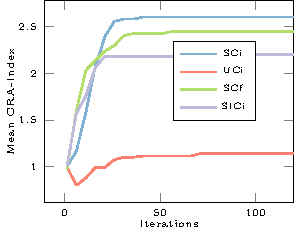
\includegraphics[width=0.45\textwidth]{single/progression-chart-a}}%
\hfill
\subcaptionbox{Multi}{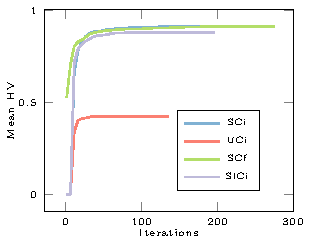
\includegraphics[width=0.48\textwidth]{multi/progression-chart-multi-a}}%
\caption{Model A.}
\end{figure}

\begin{table}%
\centering
\begin{tabular}{lccccc}
Algorithm & Min. CC & Max. CC & Avg. CC & Med. CC & SC\\
\hline
SCi & 1 & 4 & 2.4 & 2 & 150\\
UCi & 1 & 6 & 2.3 & 2 & 150\\
SCf & 1 & 4 & 2.4 & 2 & 154\\
SICi & 1 & 4 & 2.3 & 2 & 147
\end{tabular}
\caption{Minimum, maximum, average and median class count (CC) and solution count (SC) for A.}
\label{}
\end{table}

\clearpage

\begin{figure}
\centering
\subcaptionbox{Single}{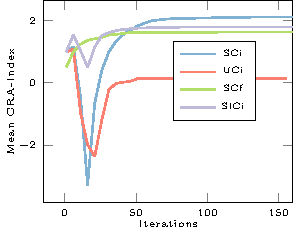
\includegraphics[width=0.45\textwidth]{single/progression-chart-b}}%
\hfill
\subcaptionbox{Multi}{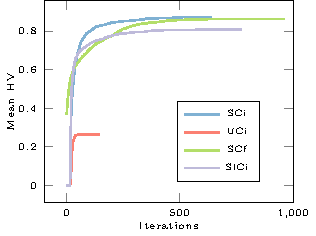
\includegraphics[width=0.48\textwidth]{multi/progression-chart-multi-b}}%
\caption{Model B.}
\end{figure}

\begin{table}%
\centering
\begin{tabular}{lccccc}
Algorithm & Min. CC & Max. CC & Avg. CC & Med. CC & SC\\
\hline
SCi & 2 & 9 & 4.5 & 4 & 1081\\
UCi & 1 & 12 & 4.4 & 4 & 97\\
SCf & 2 & 9 & 4.2 & 3 & 1225\\
SICi & 2 & 9 & 4.1 & 4 & 1259
\end{tabular}
\caption{Minimum, maximum, average and median class count (CC) and total solution count (SC) over 30 computations for B.}
\label{}
\end{table}

\clearpage

\begin{figure}
\centering
\subcaptionbox{Single}{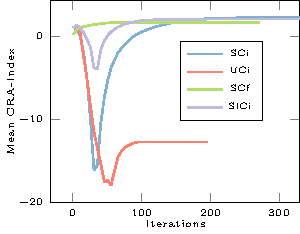
\includegraphics[width=0.47\textwidth]{single/progression-chart-c}}%
\hfill
\subcaptionbox{Multi}{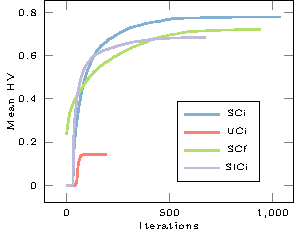
\includegraphics[width=0.46\textwidth]{multi/progression-chart-multi-c}}%
\caption{Model C.}
\end{figure}

\begin{table}%
\centering
\begin{tabular}{lccccc}
Algorithm & Min. CC & Max. CC & Avg. CC & Med. CC & SC\\
\hline
SCi & 2 & 17 & 7.6 & 8 & 2922\\
UCi & 9 & 24 & 14.3 & 14 & 100\\
SCf & 2 & 17 & 6.9 & 6 & 2992\\
SICi & 2 & 13 & 6.0 & 6 & 2981
\end{tabular}
\caption{Minimum, maximum, average and median class count (CC) and total solution count (SC) over 30 computations for C.}
\label{}
\end{table}

\clearpage

\begin{figure}
\centering
\subcaptionbox{Single}{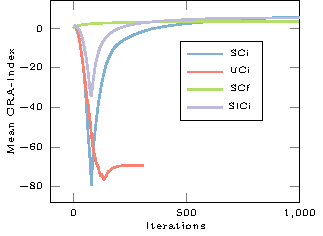
\includegraphics[width=0.49\textwidth]{single/progression-chart-d}}%
\hfill
\subcaptionbox{Multi}{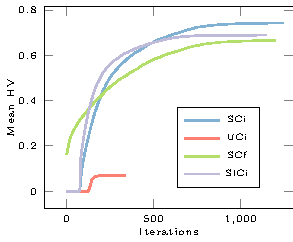
\includegraphics[width=0.44\textwidth]{multi/progression-chart-multi-d}}%
\caption{Model D.}
\end{figure}

\begin{table}%
\centering
\begin{tabular}{lccccc}
Algorithm & Min. CC & Max. CC & Avg. CC & Med. CC & SC\\
\hline
SCi & 4 & 35 & 19.5 & 19 & 3468\\
UCi & 27 & 45 & 36.0 & 36 & 78\\
SCf & 2 & 37 & 15.6 & 15 & 2982\\
SICi & 1 & 27 & 14.3 & 15 & 2987
\end{tabular}
\caption{Minimum, maximum, average and median class count (CC) and total solution count (SC) over 30 computations for D.}
\label{}
\end{table}

\clearpage

\begin{figure}
\centering
\subcaptionbox{Single}{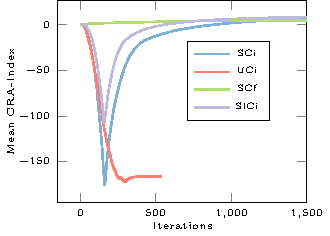
\includegraphics[width=0.47\textwidth]{single/progression-chart-e}}%
\hfill
\subcaptionbox{Multi}{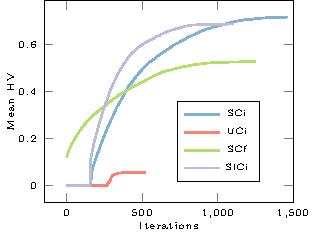
\includegraphics[width=0.46\textwidth]{multi/progression-chart-multi-e}}%
\caption{Model E.}
\end{figure}

\begin{table}%
\centering
\begin{tabular}{lccccc}
Algorithm & Min. CC & Max. CC & Avg. CC & Med. CC & SC\\
\hline
SCi & 19 & 66 & 39.6 & 39 & 2969\\
UCi & 65 & 86 & 74.1 & 75 & 76\\
SCf & 2 & 59 & 24.1 & 24 & 2997\\
SICi & 12 & 49 & 30.4 & 31 & 2993
\end{tabular}
\caption{Minimum, maximum, average and median class count (CC) and total solution count (SC) over 30 computations for E.}
\label{}
\end{table}

\end{document}